%===============================================================================
% Template Name:      SUnORE Starter Presentation template
% Template URI:       http://sunore.co.za/sunore-presentation/
% Description:        Starter Presentation template for SUnORE 
%                     Department of Industrial Engineering, 
%                     Stellenbosch University
% Version:            1.1.0
% Author:             Johan Janse van Rensburg
% Author URI:         http://johanjvrens.co.za/
% License:            MIT License
% License URI:        http://opensource.org/licenses/MIT
%===============================================================================
\documentclass[serif,10pt,aspectratio=169]{beamer}

%=================================================
% theme and color
%=================================================
\usetheme{Warsaw} %Themes http://www.hartwork.org/beamer-theme-matrix/
\definecolor{colorA}{RGB}{96, 34, 59}
\definecolor{colorB}{RGB}{140, 151, 154}
%\definecolor{secinhead}{RGB}{249,196,95}
%\definecolor{titlebg}{RGB}{51,51,51}
\setbeamercolor{structure}{fg=colorA,bg=colorB}
%\setbeamercolor{secsubsec}{fg=secinhead,bg=black}
%\setbeamercolor{frametitle}{fg=secinhead,bg=titlebg}
\beamertemplatenavigationsymbolsempty
\setbeamertemplate{caption}[numbered]
\setbeamertemplate{enumerate items}[circle]
\setbeamertemplate{itemize items}[circle]

%=================================================
% packages and new commands
%=================================================
\usepackage[ruled, linesnumbered, vlined]{algorithm2e}
\usepackage{epsfig, subcaption, amssymb,  multirow,algorithmic, amsmath, svg, booktabs}
\usepackage{marvosym}
\usepackage{xcolor}
%\usepackage[german]{babel}
\newcommand*{\superscript}[1]{\ensuremath{^{\rm #1}}}
\newcommand*{\subscript}[1]{\ensuremath{_{\rm #1}}}
%\renewcommand*{\figurename}{Abb.}
%\renewcommand{\tablename}{Tab.}
%\renewcommand{\algorithmcfname}{Algorithmus}

\usepackage[sorting = none]{biblatex}
\addbibresource{references/references.bib}
%=================================================
% thesis details (preamble)
%=================================================
\title[{\sc Metabolic Network Analysis} \hspace{3.5cm} \insertframenumber/\inserttotalframenumber]{\sc Graph theory practical course:\\
Exploration of metabolic networks}
\author[Graphen und biologische Netzwerke --- Praktikum]{{Paul Keller, Kolya Lettl, Franz Förster}}
\date{24. Feb. 2023}
\institute{Universität Leipzig \\ Fakultät Mathematik und Informatik \\ Institut für Bioinformatik}

%=================================================
% start presentation
%=================================================
\begin{document}

%========================
% title page
%========================
\begin{frame}
  \begin{center}
    %\vspace{0.1cm}
    
\includegraphics[scale=0.20]{images/logo-Leipzig.png}
  \end{center}
  \titlepage
\end{frame}

%========================
% your slides:
%========================
\begin{frame}\frametitle{WP1: amino acid production per organism}
	\begin{figure}
		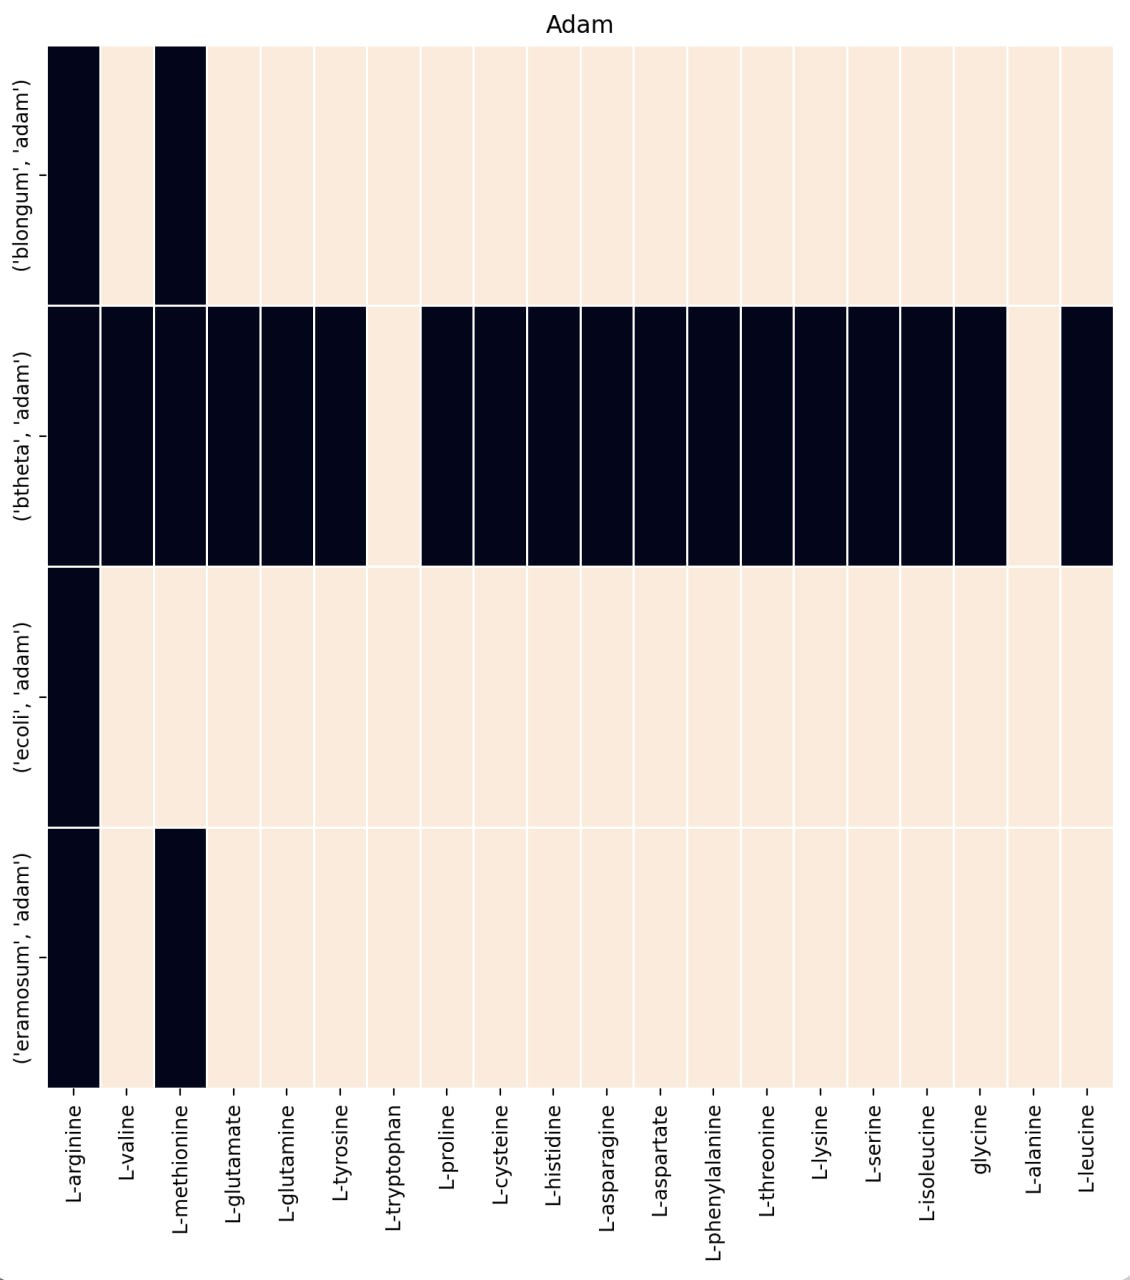
\includegraphics[height=6cm]{images/aa_presence_clean.jpg}
		\caption{Presence of amino acids dependent on organism and medium in the cleaned networks.}
	\end{figure}
\end{frame}

\begin{frame}\frametitle{WP2: number of activated reactions}
	\begin{figure}
		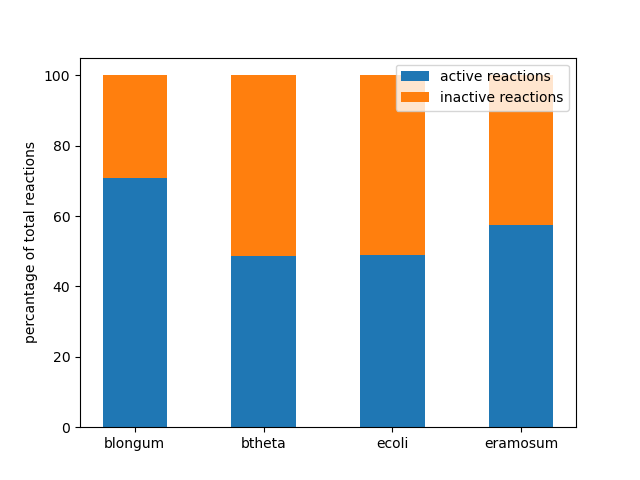
\includegraphics[height=6cm]{images/acitive_reaction_proportions_compound_threshold_1000.png}
		\caption{Proportion of active reactions (with flux) and inactive reactions. Flux calculated without compound constrains.}
	\end{figure}
\end{frame}

\begin{frame}\frametitle{WP2: biomass dependence on essential compounds}
	\begin{figure}
		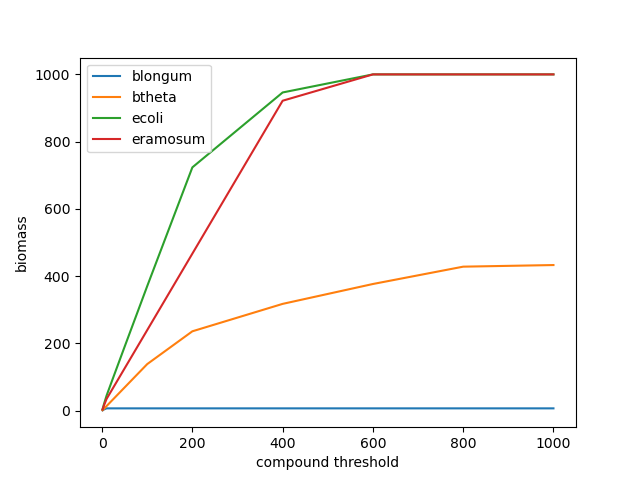
\includegraphics[height=6cm]{images/biomass.png}
		\caption{Value of the biomass function at different limitations for import reactions of essential compounds (H2O, hydronium and phosphate are always unlimited).}
	\end{figure}
\end{frame}

\begin{frame}\frametitle{WP2: activation level by compound threshold}
	\begin{columns}[t]
		\column{0.5\textwidth}
		\begin{figure}
			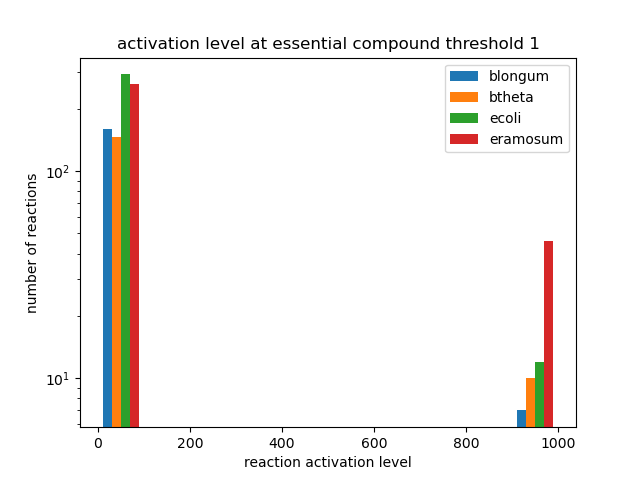
\includegraphics[width=\textwidth]{images/activation_level_by_theshold_1.png}
			\caption{Histogramm of reaction level ($|flux|$). All import reactions for essential compounds (except water, hydronium and phosphate) are limited to -1.}
		\end{figure}
	
		\column{0.5\textwidth}
		\begin{figure}
			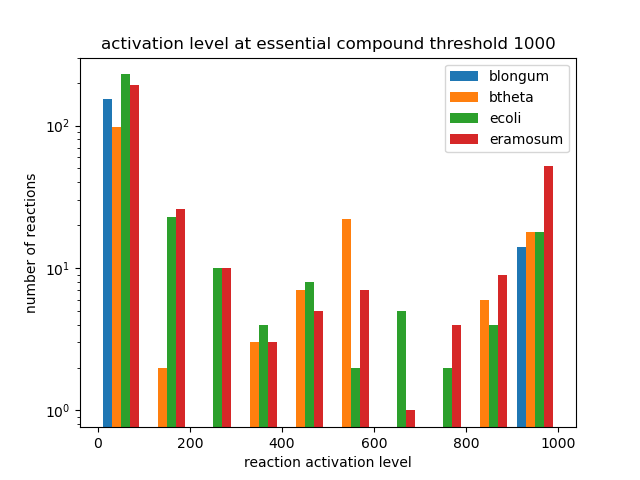
\includegraphics[width=\textwidth]{images/activation_level_by_theshold_1000.png}
			\caption{Histogramm of reaction level ($|flux|$). All import reactions for essential compounds are unlimited.}
		\end{figure}
	\end{columns}
\end{frame}

\begin{frame}\frametitle{WP2: pathway enrichment test}
	\begin{figure}
		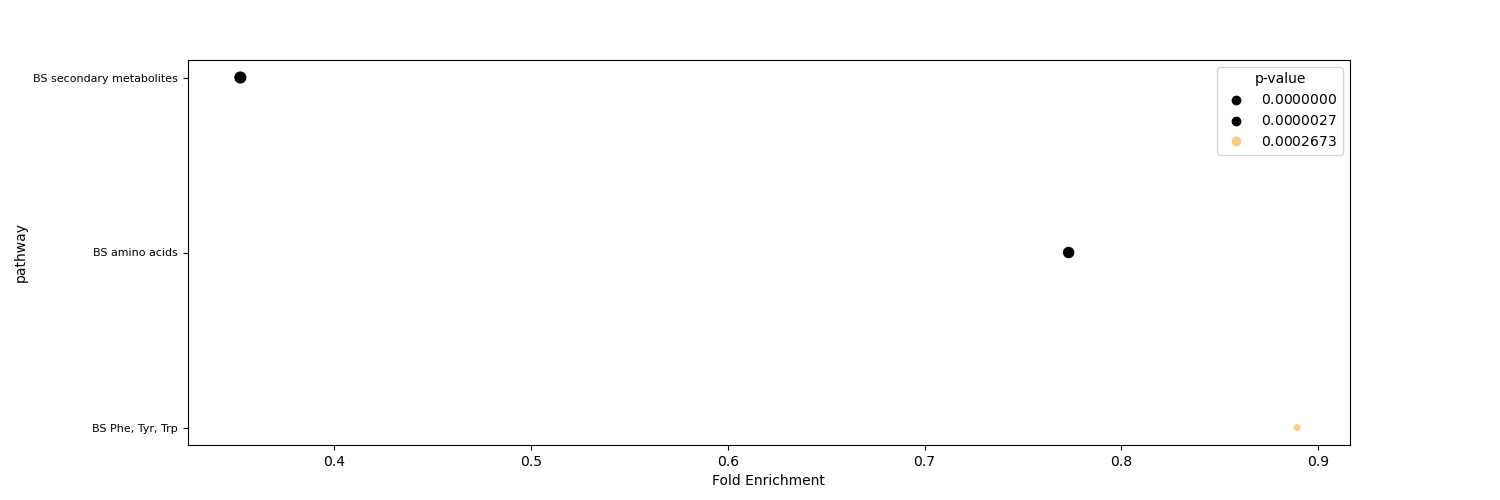
\includegraphics[width=0.95\textwidth]{images/fold_enrichment.png}
		\caption{Results of the hypergeometric enrichment test for 562 KEGG pathways. Background are all reactions in the glucose-amino acid graph and foreground are all reactions with flux.}
	\end{figure}
\end{frame}

\begin{frame}\frametitle{WP3: component size}
	\begin{columns}[t]
		\column{0.5\textwidth}
		\begin{figure}
			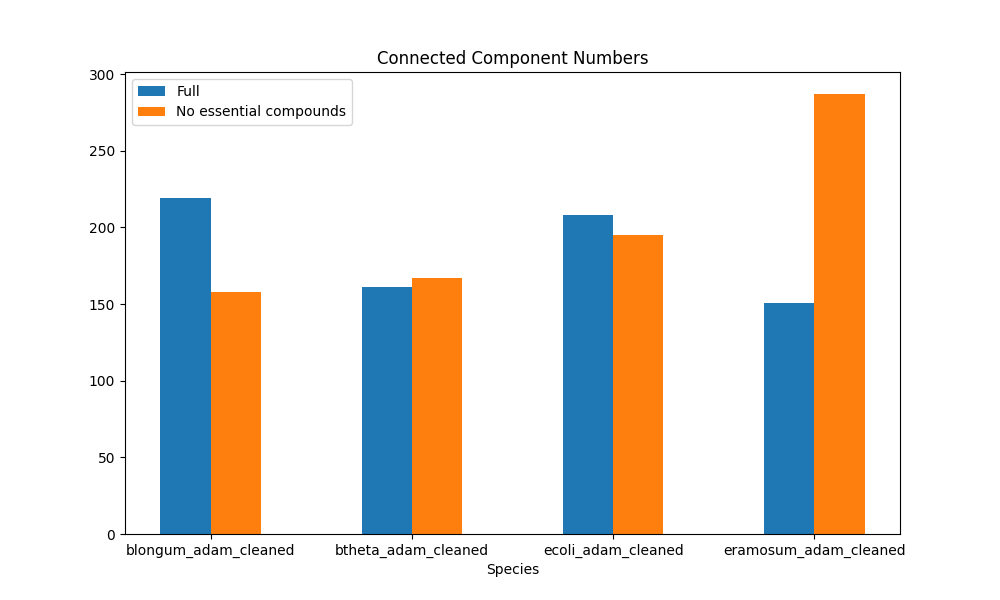
\includegraphics[height=4cm]{images/04_component_numbers.png}
			\caption{Number of connected components for each atom combined per species. Results are compared between original ATN and an ATN where all essential compounds are removed.}
		\end{figure}
		\column{0.5\textwidth}
		\begin{figure}
			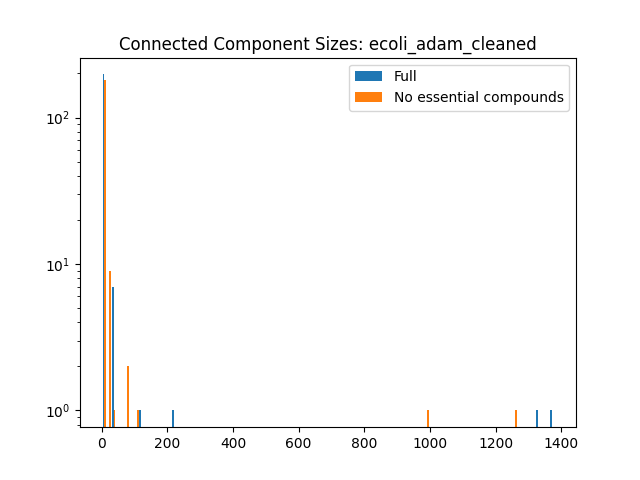
\includegraphics[height=4cm]{images/ecoli_adam_cleaned.png}
			\caption{Histogram of the connected components sizes.  Results are compared between original ATN and an ATN where all essential compounds are removed.}
	\end{figure}
	\end{columns}
\end{frame}

\begin{frame}\frametitle{WP3: endpoint analysis}
	\begin{figure}
		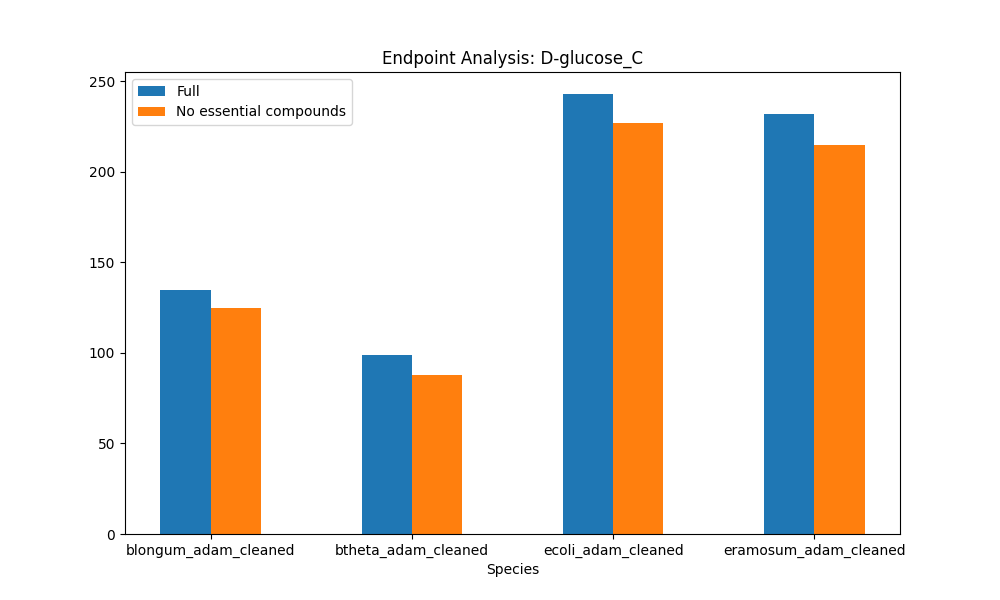
\includegraphics[height=6cm]{images/01_endpoint_analysis.png}
		\caption{Number of endpoints (compounds not used in further reactions) compared between the species.  Results are compared between original ATN and an ATN where all essential compounds are removed.}
	\end{figure}
\end{frame}

%========================
% bibliography
%========================


%=================================================
% end presentation
%=================================================
\end{document}